\chapter{Sprint 3 -- Connected Mode and SQL Server Integration}


% ─────────────────────────────────────────────
\section*{Introduction}
\addcontentsline{toc}{section}{Introduction}
% ─────────────────────────────────────────────


\paragraph{}This chapter presents Sprint 3, which spanned four weeks and extended the generator from a standalone synthetic tool
into a connected assistant capable of working with an existing Longview SQL Server environment.
The objective of this sprint was to allow QA engineers to connect to a database, browse selected
reference entities, choose the subset of data to reuse, and generate additional pre-BCP records
anchored to that database state. This mode preserves the same output objective as standalone mode:
a coherent SQL loading script, but it builds part of the dataset from existing accounts or securities
instead of generating everything from scratch.

\paragraph{}The sprint therefore focused on three major concerns: secure database access, selective data
grabbing, and connected generation. The implementation introduced a dedicated
\texttt{DatabaseModule}, a \texttt{ConnectedController}, a \texttt{DatabaseService} for SQL Server
connectivity, and a \texttt{ConnectedGeneratorService} that reuses the entity generation services
implemented in Sprint 2 while adapting them to grabbed database records.

\paragraph{}The chapter follows the same sprint structure as the previous implementation chapter:
sprint backlog, sprint specification, sprint design, implementation, sprint review and validation,
then conclusion. To avoid repetition, it focuses only on what connected mode adds to the
standalone generation engine.


% ─────────────────────────────────────────────
\section{Sprint Backlog}
% ─────────────────────────────────────────────


\paragraph{}Sprint 3 targeted the connected-mode user story from the product backlog: connecting to a
Longview SQL Server instance in read-only mode and generating coherent records from existing
reference data. The sprint backlog is presented in Table~\ref{tab:sprint3-backlog}.

\renewcommand{\arraystretch}{1.35}
\begin{longtable}{|Q{0.06\linewidth}|P{0.30\linewidth}|P{0.42\linewidth}|Q{0.12\linewidth}|}
\caption{Sprint 3 backlog}
\label{tab:sprint3-backlog} \\
\hline
\textbf{ID} & \textbf{Task} & \textbf{Description} & \textbf{Estimate} \\
\hline
\endfirsthead
\multicolumn{4}{r}{\tablename\ \thetable{} -- \textit{continued from previous page}} \\
\hline
\textbf{ID} & \textbf{Task} & \textbf{Description} & \textbf{Estimate} \\
\hline
\endhead
\hline
\multicolumn{4}{r}{\textit{continued on next page}} \\
\endfoot
\hline
\endlastfoot
T3-1 & Implement SQL Server connection service & Create a service able to test, open, reuse, and close SQL Server connections using either Windows authentication or SQL authentication. & 2 days \\
\hline
T3-2 & Implement connected backend API & Add endpoints for testing the connection, connecting, disconnecting, fetching allowed tables, grabbing account groups, grabbing accounts, previewing generation, and generating the final SQL script. & 2 days \\
\hline
T3-3 & Implement data grabbing logic & Allow users to select existing account groups, accounts, and securities, then transform database rows into DTO-compatible records for the generation pipeline. & 2 days \\
\hline
T3-4 & Implement connected generation service & Build a connected orchestrator that combines grabbed records with newly generated dependent records such as prices, positions, orders, models, and executions. & 2 days \\
\hline
T3-5 & Implement connected frontend workflow & Build the connection, data grabber, configuration, preview, and generation steps under the \texttt{/connected} route. & 2 days \\
\hline
T3-6 & Add safeguards and validation & Restrict raw table fetching to approved tables, require a live connection before connected actions, and validate generated output before writing files. & 1 day \\
\hline
\end{longtable}


% ─────────────────────────────────────────────
\section{Sprint Specification}
\paragraph{}Connected mode extends the standalone generation use case by adding a database preparation
phase. Before generation, the QA engineer connects to SQL Server and selects existing accounts or
securities that will serve as anchors for the generated scenario.

\renewcommand{\arraystretch}{1.15}
\begin{longtable}{|P{0.24\linewidth}|P{0.66\linewidth}|}
\caption{Textual description of the connected generation use case}
\label{tab:connected-usecase-description} \\
\hline
\textbf{Element} & \textbf{Description} \\
\hline
\endfirsthead
\multicolumn{2}{r}{\tablename\ \thetable{} -- \textit{continued from previous page}} \\
\hline
\textbf{Element} & \textbf{Description} \\
\hline
\endhead
\hline
\multicolumn{2}{r}{\textit{continued on next page}} \\
\endfoot
\hline
\endlastfoot
Use case & Generate a SQL loading script anchored to existing Longview data. \\
\hline
Actor & QA Engineer. \\
\hline
Preconditions & A SQL Server instance is reachable and the QA engineer has valid read-only connection information. \\
\hline
Postconditions & Existing records are reused as anchors and a coherent \texttt{load\_test\_data.sql} file is generated. \\
\hline
Nominal scenario &
\begin{enumerate}[leftmargin=*,nosep]
    \item The QA engineer enters SQL Server connection information.
    \item The system tests and opens the connection.
    \item The QA engineer grabs existing accounts, account groups, or securities.
    \item The system infers the connected generation case from the selected data.
    \item The QA engineer configures only the missing or dependent records.
    \item The system previews the result, then generates the final SQL script.
\end{enumerate} \\
\hline
Exception scenario &
\begin{itemize}[leftmargin=*,nosep]
    \item If connection fails, the workflow stops before data grabbing.
    \item If no compatible data is selected, preview and generation are rejected.
    \item If a selected table is not allowed, the backend refuses the request.
\end{itemize} \\
\hline
\end{longtable}


\section{Sprint Design}
% ─────────────────────────────────────────────


\subsection{Connected Mode Use Case Diagram}

\paragraph{}Figure~\ref{fig:usecase-connected} presents the connected mode use cases implemented in this
sprint. This mode adds database-specific actions such as testing the connection, connecting with
Windows authentication or SQL Server authentication, grabbing account and security reference data,
and disconnecting from SQL Server. The SQL Server actor is involved only through read-only
operations.

\begin{figure}[H]
\centering
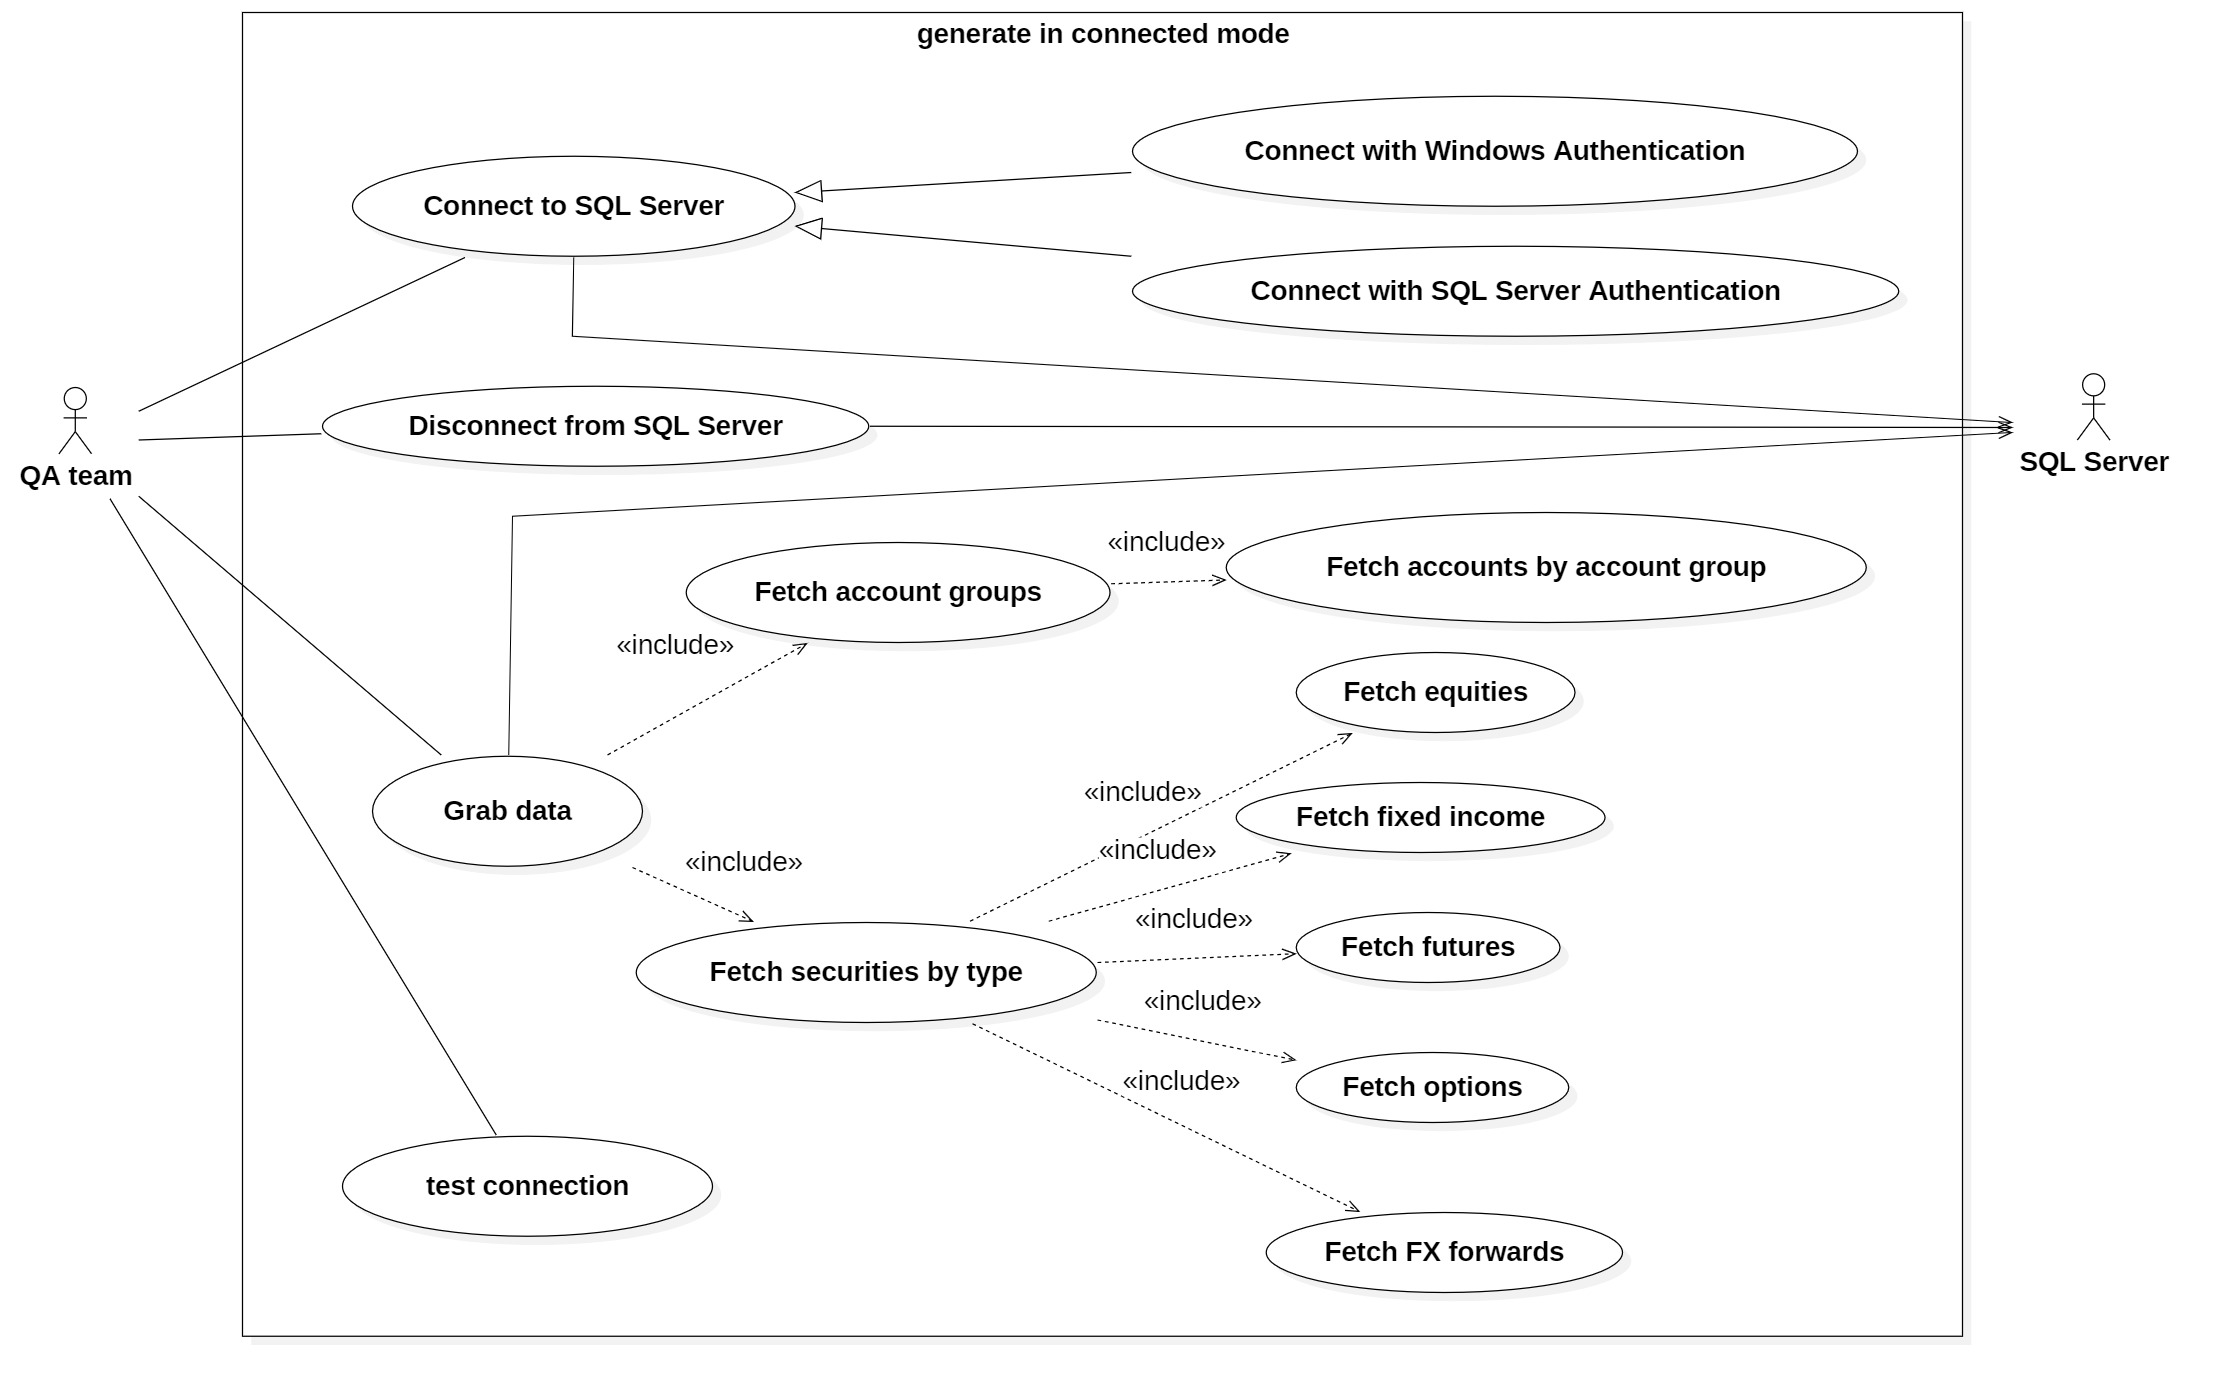
\includegraphics[width=1\textwidth]{img/usecase-connected-mode.jpg}
\caption{Connected mode use case diagram}
\label{fig:usecase-connected}
\end{figure}

\subsection{Connected Mode Architecture}

\paragraph{}Connected mode is built as an extension of the generation engine rather than as a separate
generator. The backend introduces the \texttt{DatabaseModule}, which groups the
\texttt{ConnectedController}, the \texttt{DatabaseService}, and the
\texttt{ConnectedGeneratorService}. The \texttt{DatabaseService} owns the SQL Server connection pool,
while the connected generator receives grabbed data, prepares the connected dataset, validates it,
and delegates SQL script assembly to the same \texttt{SqlScriptGeneratorService} used by standalone
mode.

\paragraph{}This architecture avoids duplication: connected mode reuses the account, account group,
hierarchy, security, price, model, position, order, execution, validator, and SQL script services
implemented during Sprint 2. The connected-specific layer is responsible only for selecting the
source data, mapping database rows to generator DTOs, and deciding which dependent records must be
generated according to the selected grab mode.

\begin{figure}[htbp]
\centering
%\includegraphics[width=1\textwidth]{img/ch5-connected-architecture.pdf}
\caption{Architecture of the connected mode}
\label{fig:ch5-connected-architecture}
\end{figure}

\subsection{Connected Workflow}

\paragraph{}The frontend implements connected mode as a five-step workflow:
\texttt{/connected/connection}, \texttt{/connected/data-grabber},
\texttt{/connected/configuration}, \texttt{/connected/preview}, and
\texttt{/connected/generation}. This sequence reflects the additional constraints introduced by
database usage: the user must connect first, then grab reference data, then configure only the
records that still need to be generated.

\renewcommand{\arraystretch}{1.3}
\begin{longtable}{|P{0.18\linewidth}|P{0.28\linewidth}|P{0.44\linewidth}|}
\caption{Connected mode workflow}
\label{tab:connected-workflow} \\
\hline
\textbf{Step} & \textbf{Route} & \textbf{Purpose} \\
\hline
\endfirsthead
\multicolumn{3}{r}{\tablename\ \thetable{} -- \textit{continued from previous page}} \\
\hline
\textbf{Step} & \textbf{Route} & \textbf{Purpose} \\
\hline
\endhead
\hline
\multicolumn{3}{r}{\textit{continued on next page}} \\
\endfoot
\hline
\endlastfoot
Connection & \texttt{/connected/connection} & Enter SQL Server details, choose authentication mode, test the connection, and open the active backend connection. \\
\hline
Data grabber & \texttt{/connected/data-grabber} & Browse available account groups, accounts, and security buffer tables, then select the records that will anchor generation. \\
\hline
Configuration & \texttt{/connected/configuration} & Configure generated complements such as accounts, securities, prices, models, positions, orders, and executions. \\
\hline
Preview & \texttt{/connected/preview} & Run the backend generation rules without writing files and display estimated rows, summaries, warnings, and samples. \\
\hline
Generation & \texttt{/connected/generation} & Generate the connected dataset, assemble the SQL script, and download \texttt{load\_test\_data.sql}. \\
\hline
\end{longtable}

\begin{figure}[htbp]
\centering
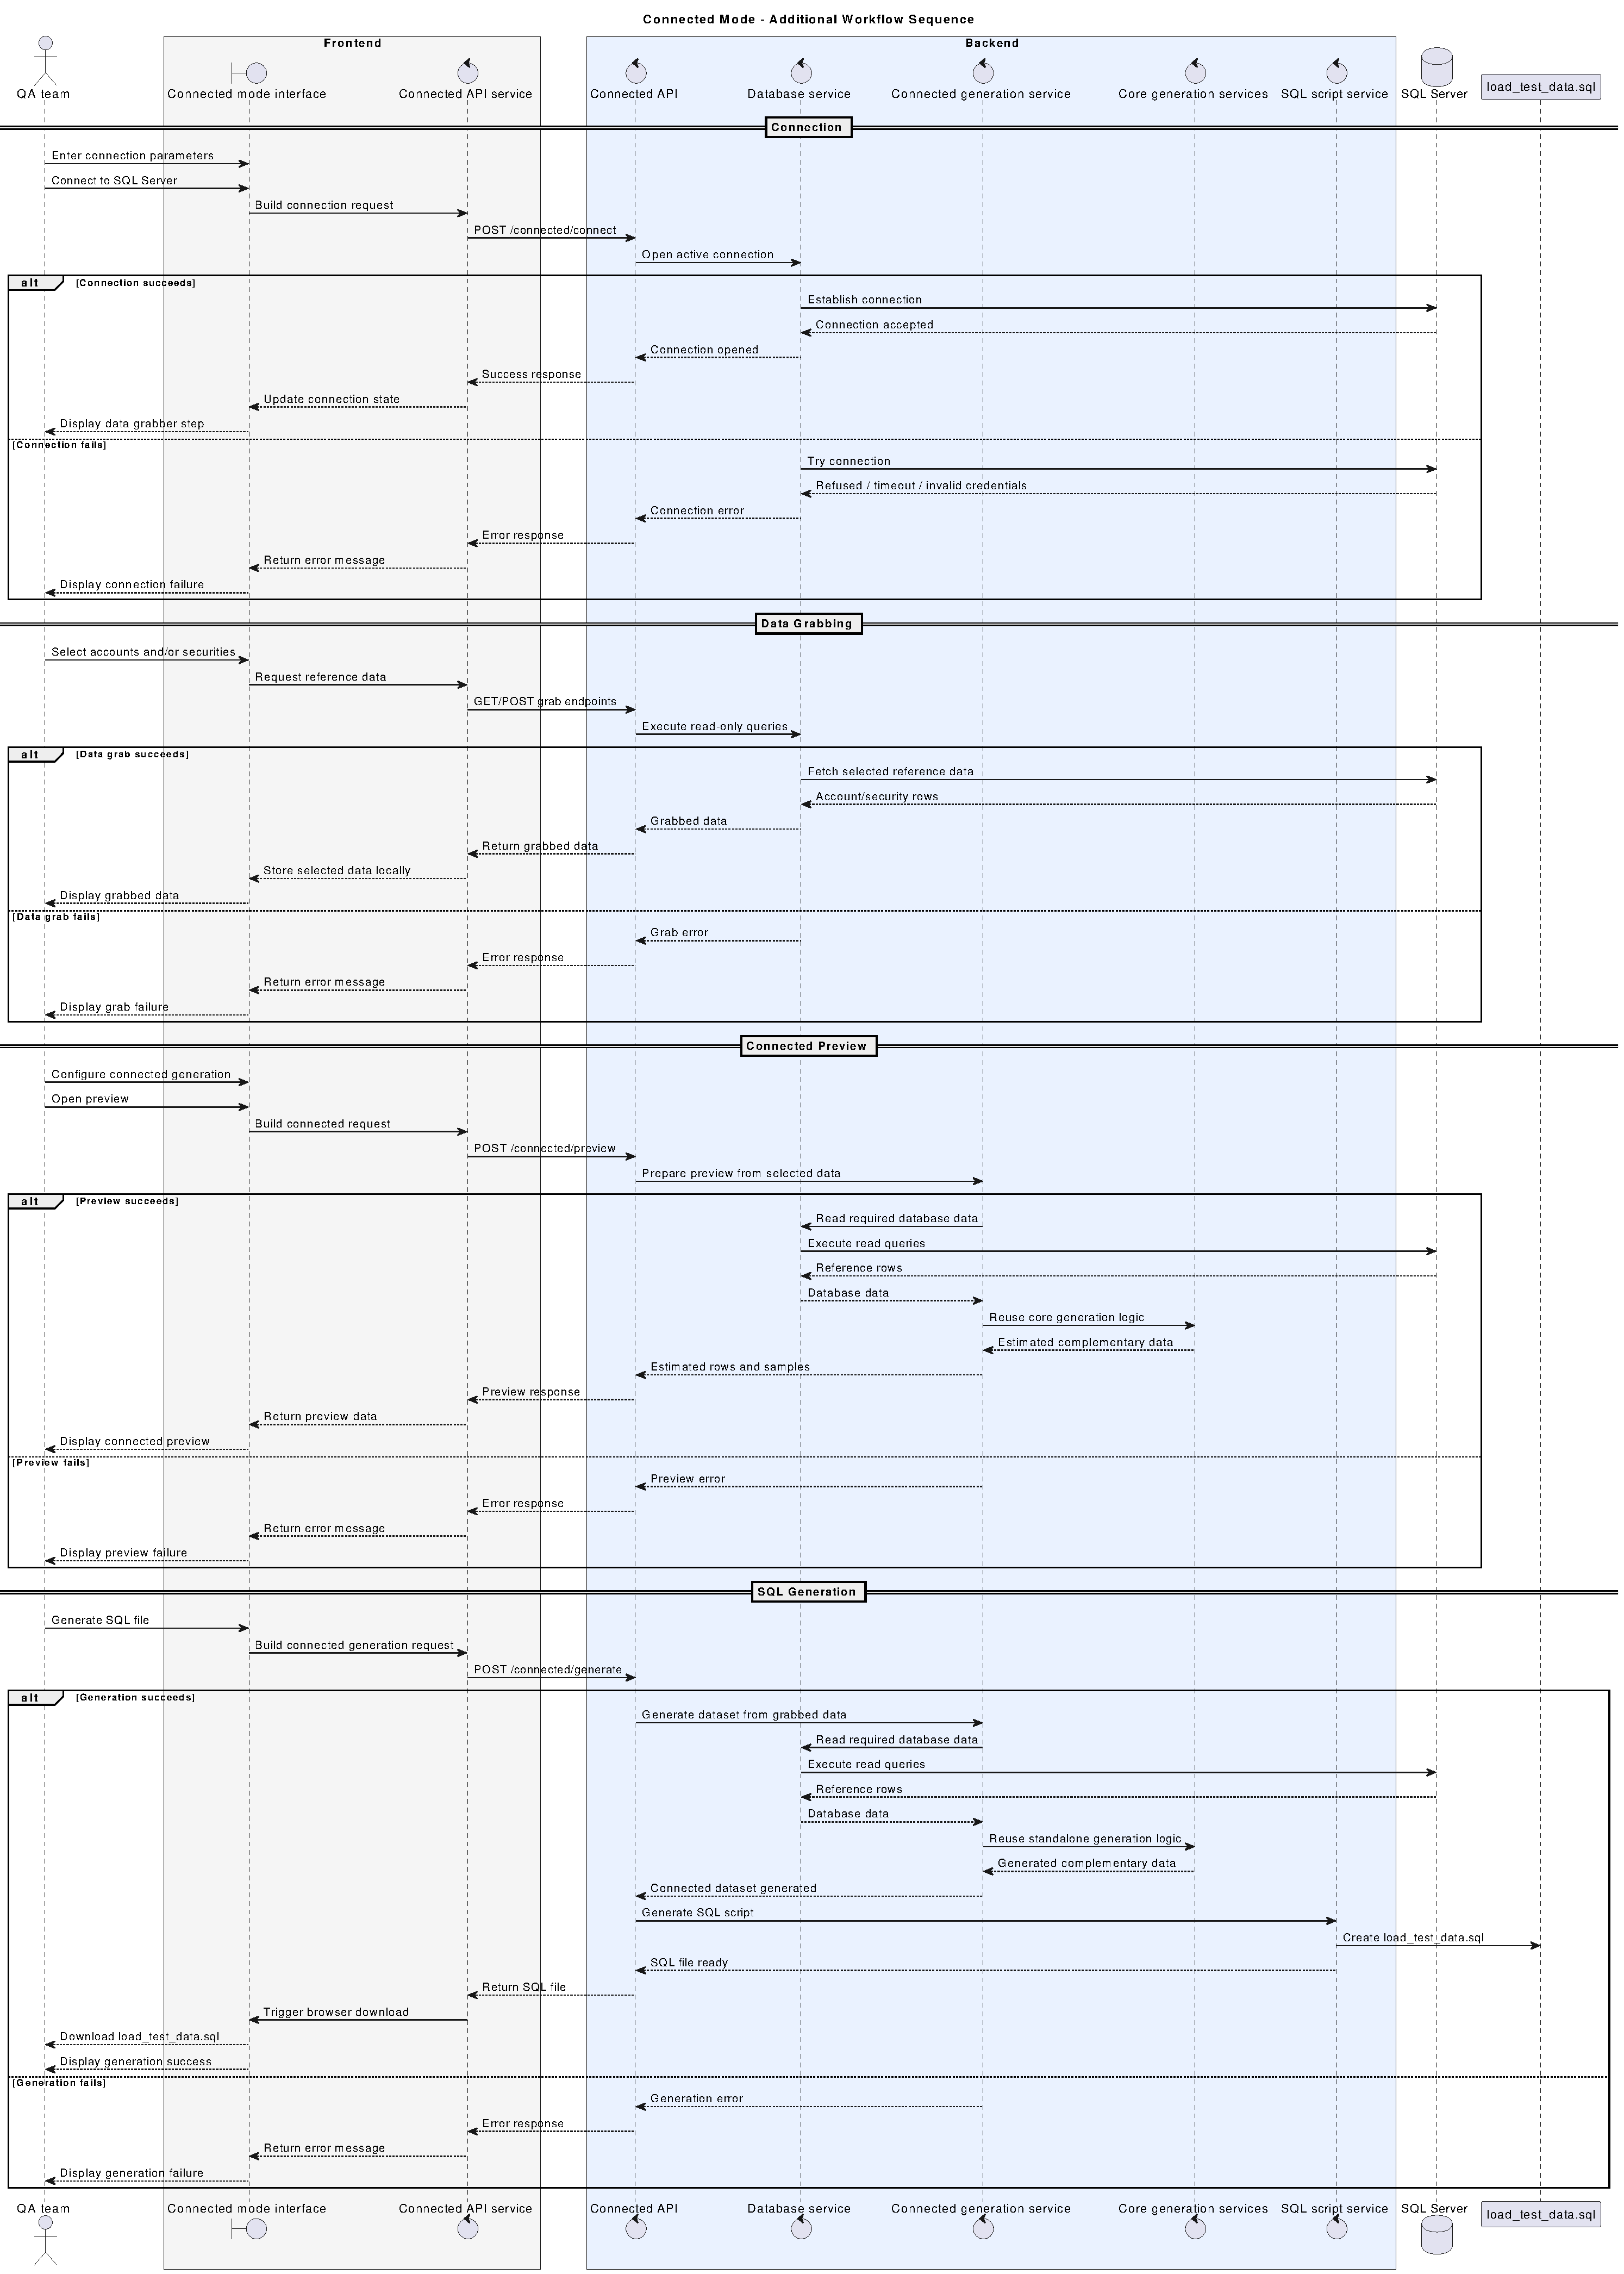
\includegraphics[width=1\textwidth]{img/sequence-connected-mode.pdf}
\caption{Connected mode workflow sequence}
\label{fig:ch5-connected-sequence}
\end{figure}

\paragraph{}Figure~\ref{fig:ch5-connected-sequence} details the additional exchanges introduced by
connected mode. Compared with standalone generation, the workflow begins with a SQL Server
connection request, continues with read-only data grabbing, and only then reaches preview and SQL
generation. The connected API delegates database access to \texttt{DatabaseService}, while
\texttt{ConnectedGeneratorService} prepares the selected account and security context before reusing
the core generation services.

\paragraph{}The alternate branches in the sequence diagram show how the application handles connection
errors, failed data grabs, preview errors, and generation failures. These paths are important
because connected mode depends on external database availability; every backend failure is returned
as a structured frontend message instead of leaving the user in an ambiguous state.

\subsection{Grab Modes}

\paragraph{}Connected generation supports three cases, referred to in the implementation as
\texttt{grabMode}. The grab mode is inferred automatically on the frontend from the selected data
and is sent to the backend as part of the connected generation request.

\renewcommand{\arraystretch}{1.3}
\begin{longtable}{|P{0.24\linewidth}|P{0.32\linewidth}|P{0.34\linewidth}|}
\caption{Connected generation grab modes}
\label{tab:grab-modes} \\
\hline
\textbf{Grab mode} & \textbf{Grabbed data} & \textbf{Generated complement} \\
\hline
\endfirsthead
\multicolumn{3}{r}{\tablename\ \thetable{} -- \textit{continued from previous page}} \\
\hline
\textbf{Grab mode} & \textbf{Grabbed data} & \textbf{Generated complement} \\
\hline
\endhead
\hline
\multicolumn{3}{r}{\textit{continued on next page}} \\
\endfoot
\hline
\endlastfoot
\texttt{accounts} & Existing accounts or account groups & Securities can be generated, then prices and dependent portfolio/trading records can be generated from the grabbed account universe. \\
\hline
\texttt{securities} & Existing securities & Accounts can be generated, then prices and dependent records can be generated from the grabbed security universe. \\
\hline
\shortstack[l]{\texttt{accounts\_and\_}\\\texttt{securities}} & Existing accounts and securities & Only dependent records are generated, such as prices, models, positions, orders, and executions. \\
\hline
\end{longtable}


% ─────────────────────────────────────────────
\section{Implementation}
\paragraph{}This section presents only the implementation elements added by connected mode. The core
generation services, validation rules, and SQL assembly mechanism were already introduced in
Sprint 2; here, the focus is on SQL Server access, controlled data grabbing, connected orchestration,
and connected preview/generation endpoints.
% ─────────────────────────────────────────────


\subsection{SQL Server Connection Service}

\paragraph{}The \texttt{DatabaseService} supports two authentication modes. For Windows authentication, it
uses the \texttt{mssql/msnodesqlv8} driver and builds an ODBC connection string containing the
server name, database name, selected ODBC driver, and trusted connection option. For SQL
authentication, it uses the standard \texttt{mssql} driver with an explicit username and password.
Both modes apply a configurable connection timeout and set \texttt{TrustServerCertificate} to allow
connections to internal development databases.

\paragraph{}The service exposes three core operations. The \texttt{testConnection()} method opens a temporary
connection, reports success or failure, and closes the pool immediately. The \texttt{connect()} method
opens and stores the active pool used by later grabber and generation requests. The
\texttt{disconnect()} method closes the active pool and clears the connection state. This separation
allows the user to test credentials before committing to a connected session.

\begin{figure}[htbp]
\centering
%\includegraphics[width=0.95\textwidth]{img/ch5-connection-step.pdf}
\caption{Connected mode -- SQL Server connection step}
\label{fig:ch5-connection-step}
\end{figure}

\subsection{Connected Backend API}

\paragraph{}The \texttt{ConnectedController} exposes the connected API under the \texttt{/connected} prefix.
Table~\ref{tab:connected-api} summarizes the main endpoints implemented during this sprint.

\renewcommand{\arraystretch}{1.3}
\begin{longtable}{|P{0.28\linewidth}|Q{0.18\linewidth}|P{0.44\linewidth}|}
\caption{Connected mode backend endpoints}
\label{tab:connected-api} \\
\hline
\textbf{Endpoint} & \textbf{Method} & \textbf{Role} \\
\hline
\endfirsthead
\multicolumn{3}{r}{\tablename\ \thetable{} -- \textit{continued from previous page}} \\
\hline
\textbf{Endpoint} & \textbf{Method} & \textbf{Role} \\
\hline
\endhead
\hline
\multicolumn{3}{r}{\textit{continued on next page}} \\
\endfoot
\hline
\endlastfoot
\texttt{/connected/test} & POST & Test SQL Server credentials and return connection logs. \\
\hline
\texttt{/connected/connect} & POST & Open the active SQL Server connection pool. \\
\hline
\texttt{/connected/disconnect} & POST & Close the active SQL Server connection. \\
\hline
\shortstack[l]{\texttt{/connected/grab/}\\\texttt{account-groups}} & GET & Return available account group names from the account hierarchy. \\
\hline
\shortstack[l]{\texttt{/connected/grab/}\\\texttt{accounts}} & POST & Return accounts linked to selected account groups. \\
\hline
\texttt{/connected/fetch/:table} & GET & Fetch rows from an approved table for the security grabber. \\
\hline
\texttt{/connected/preview} & POST & Prepare connected artifacts and return row estimates and sample rows without writing files. \\
\hline
\texttt{/connected/generate} & POST & Generate the connected dataset and download the final SQL script. \\
\hline
\end{longtable}

\subsection{Data Grabber}

\paragraph{}The data grabber provides a controlled read-only browsing layer on top of the SQL Server
connection. Account groups are retrieved from \texttt{account\_hierarchy\_map} by joining parent and
child accounts, while selected account groups can be expanded into their child accounts. Securities
are retrieved from approved pre-BCP tables such as \texttt{pre\_bcp\_eqty\_invest\_buffer},
\texttt{pre\_bcp\_fixinc\_mnymkt\_buffer}, \texttt{pre\_bcp\_futures\_buffer},
\texttt{pre\_bcp\_option\_buffer}, \texttt{pre\_bcp\_fx\_forward\_buffer}, and
\texttt{pre\_bcp\_generic\_buffer}.

\paragraph{}The backend deliberately restricts raw fetching through an \texttt{ALLOWED\_TABLES} list. This
prevents arbitrary table access through the \texttt{/connected/fetch/:table} endpoint and keeps the
feature aligned with its purpose: browsing only the Longview reference and pre-BCP tables needed
for test data generation.

\begin{figure}[htbp]
\centering
%\includegraphics[width=0.95\textwidth]{img/ch5-data-grabber-step.pdf}
\caption{Connected mode -- Data grabber step}
\label{fig:ch5-data-grabber-step}
\end{figure}

\subsection{Connected Generator Service}

\paragraph{}The \texttt{ConnectedGeneratorService} is the orchestrator for connected mode. It first validates
the request, requiring a reference date and ensuring that the grabbed data matches the selected
\texttt{grabMode}. It then prepares a set of connected artifacts containing accounts, account groups,
hierarchies, models, securities, prices, positions, proposed orders, group orders, executions, and
warnings.

\paragraph{}When existing account rows are used, the service maps them into \texttt{AccountDto} records. It
normalises dates into the expected \texttt{YYYYMMDD} format, extracts account identifiers and short
names from several possible column names, and fills missing optional values with safe defaults such
as \texttt{CONNECTED\_DB} as source system. When securities are grabbed, each selected security subtype
is filtered by \texttt{client\_security\_id}; fixed income child schedules are also fetched when fixed
income securities are selected.

\paragraph{}After the grabbed data is prepared, the service generates only the necessary complements. For
example, if accounts are grabbed but securities are not, the security service generates the selected
security quantities. If securities are grabbed but accounts are not, the account service generates
the requested account set. If both are grabbed, the service skips master-data generation and only
generates dependent records such as prices, positions, models, orders, and executions.

\subsection{Preview and Generation}

\paragraph{}The preview endpoint runs the same preparation logic as generation but does not write files.
Instead, it returns a structured response containing estimated rows, counts per entity type, sample
rows for manual inspection, and warnings collected during safe queries. This gives the user a final
checkpoint before downloading the SQL script.

\paragraph{}The generation endpoint calls the same connected preparation logic, validates the connected
dataset through the \texttt{ValidatorService}, then delegates to the
\texttt{SqlScriptGeneratorService} to build \texttt{load\_test\_data.sql}. The generated script is
returned as a file download from the browser.

\begin{figure}[htbp]
\centering
%\includegraphics[width=0.95\textwidth]{img/ch5-connected-preview.pdf}
\caption{Connected mode -- Preview step}
\label{fig:ch5-connected-preview}
\end{figure}

\begin{figure}[htbp]
\centering
%\includegraphics[width=0.95\textwidth]{img/ch5-connected-result.pdf}
\caption{Connected mode -- Generation result}
\label{fig:ch5-connected-result}
\end{figure}


% ─────────────────────────────────────────────
\section{Sprint Review and Validation}
% ─────────────────────────────────────────────


\paragraph{}Sprint 3 produced the complete connected workflow from connection to SQL script download.
The main validation activities are summarized in Table~\ref{tab:sprint3-validation}.

\renewcommand{\arraystretch}{1.3}
\begin{longtable}{|P{0.24\linewidth}|P{0.40\linewidth}|P{0.26\linewidth}|}
\caption{Sprint 3 validation summary}
\label{tab:sprint3-validation} \\
\hline
\textbf{Validated element} & \textbf{Verification performed} & \textbf{Result} \\
\hline
\endfirsthead
\multicolumn{3}{r}{\tablename\ \thetable{} -- \textit{continued from previous page}} \\
\hline
\textbf{Validated element} & \textbf{Verification performed} & \textbf{Result} \\
\hline
\endhead
\hline
\multicolumn{3}{r}{\textit{continued on next page}} \\
\endfoot
\hline
\endlastfoot
Connection handling & Tested the separate connection test, connect, and disconnect API paths. & The backend can open a temporary pool for testing and a persistent pool for connected sessions. \\
\hline
Read-only data access & Checked that the controller only exposes \texttt{SELECT} queries and restricts raw table fetching to \texttt{ALLOWED\_TABLES}. & Connected mode does not expose write, update, or delete operations against SQL Server. \\
\hline
Grab mode coherence & Submitted requests for accounts-only, securities-only, and accounts-and-securities cases. & The backend requires the corresponding grabbed data and rejects incoherent requests. \\
\hline
Preview behavior & Used \texttt{/connected/preview} before generation. & The response returns estimated rows, summary counts, sample rows, and warnings without writing files. \\
\hline
Output generation & Generated the final SQL script from connected artifacts. & The connected dataset was validated and assembled into \texttt{load\_test\_data.sql}. \\
\hline
\end{longtable}

\paragraph{}The major technical difficulty of this sprint was reconciling existing database records with the
strict DTO contracts from Sprint 1. Database column names can differ depending on whether the data
comes from live tables or pre-BCP buffer tables, so the connected generator includes mapping helpers
that accept several candidate column names and fall back to safe default values when optional fields
are missing.


% ─────────────────────────────────────────────
\section*{Conclusion}
\addcontentsline{toc}{section}{Conclusion}
% ─────────────────────────────────────────────


\paragraph{}This chapter presented Sprint 3, which delivered the connected mode of the Longview Test Data
Generator. The sprint introduced SQL Server connectivity, controlled data grabbing, connected
preview, and connected SQL generation. The implementation reused the core services from Sprint 2
while adding a new orchestration layer able to combine existing Longview records with newly
generated dependent data. The connected mode therefore gives QA engineers a more realistic testing
workflow: they can anchor generated scenarios to an existing database state while still receiving a
ready-to-load SQL script. The following chapter presents Sprint 4, which adds optional Large
Language Model enrichment to improve the realism of generated financial labels and descriptions.
